\section{Composing declarative static analyzers}

In this section, we propose a gneralized approach for performing declarative
static analysis for a multilingual program.

\subsection{Syntax of data-fact and rule}

First, we define the syntax of data-fact and rule, which is fairly simple.

\[e := num | string\]
\[df := p(\overline{e})\]
\[r := df :- \overline{(not)? df}\]

e stands for an element, and is either number or string.  df stands for
data-fact, and it is an ordered tuple of elements.  r stands for rule, and it
denotes how one rule can be derived from another data-facts.  It states that
LHS data-fact(the data-fact before the symbol ":-") holds if all RHS data-facts
(data-facts after the symbol ":-") without "not" notation holds, and all RHS
data-facts with "not" notation does not hold.  (? Note that recursion is
permitted, that is, a data-fact can depend on itself.  The exception is the
recursion with odd number of negation, that is, the rule such as "p(x) :- not
p(x)" is not valid. ?)

\subsection{Static analyzer for one languge}

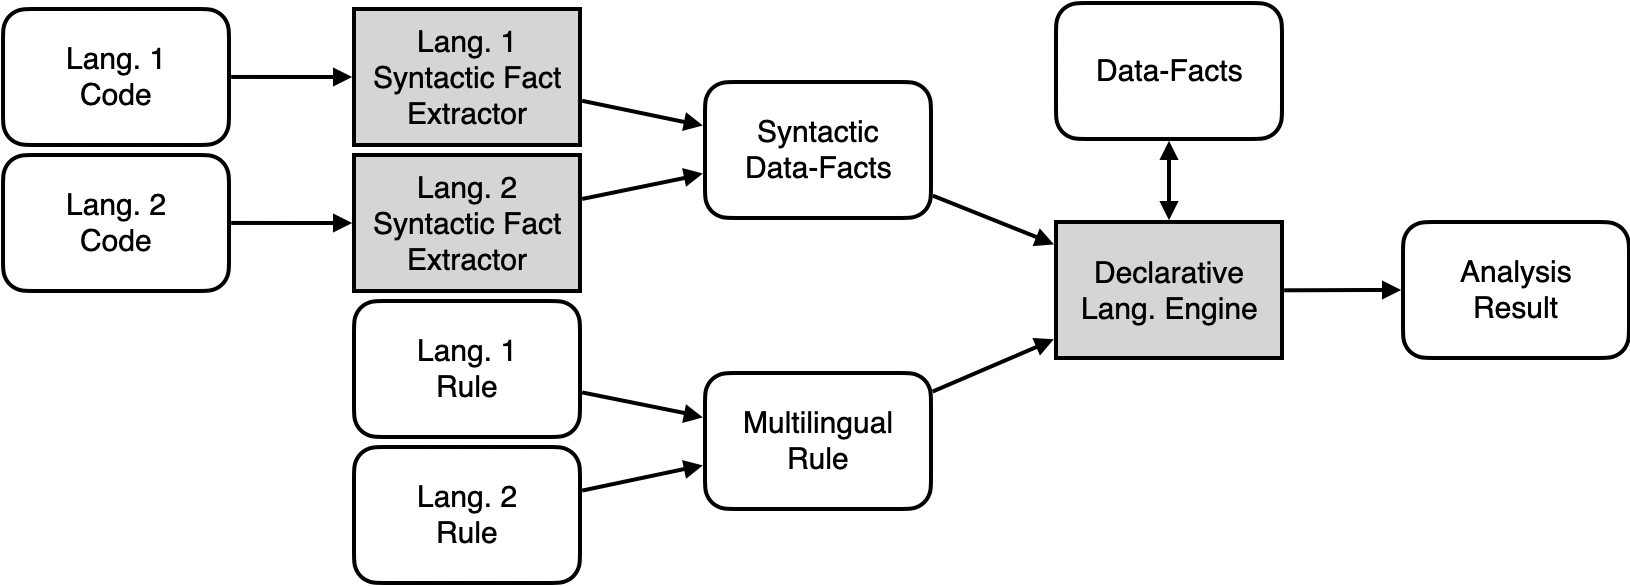
\includegraphics[width=0.5\textwidth]{img/overview}

Above figure illustrate the overview of how declarative style analysis works for
one language works. The analysis mainly
consists of three steps. First, the language is converted into a syntactic
data-facts. Second, the rules that would generate new facts are defined, and
these rules correspond to the actual implementation of the analysis. Finally, the
declarative language engine is executed with the given data-facts and rules,
giving the analysis result as an output in form of data fact.

\textbf{Extracting syntactic data-fact}
The first step is to extract syntactic data-facts from the source code.
The example of syntactic data-facts would be data-facts about certain
AST node, or parent-child relationship between nodes. For example, consider
the following code:

1 int x = 42 + 43;

We can define a data-fact of the form "expr(i, s)", which is a 2-dimensional
tuple of a number indicationg the expression id and the string representation
of that expression in the source code.  Therefore, we can extract the following
set of expr data-facts: expr(0, "42"), expr(1, "43"), and expr(2, "42 + 43"),
which indicates "42" is the 0-th expression, "43" is the 1-st, and the "42 +
43" is th 2-nd.  Another example of syntactic data-fact would be "subexpr(i, j,
k)", which is a 3-dimensional data-fact that indicates that the i-th expression
has j-th expression k-th expression. For example, we can extract the rule
subexpr(2, 0, 0) and subexpr(2, 1, 1).

In a sense, these syntactic data-facts can be viewed as building blocks for IR
of two languages.  Compared to other IRs, this declrative style of IR has a few
advantages. First, extracting in this format does not require consideration of
semantics.  It imposes almost no overhead beyond parsing the source code.
Second, the syntactic data-facts can be utilzed easily in any other kind of
analysis, since they are basically also a data-fact that can be simply
manipulated by defining new rules.  This also means that there is no need to
re-extract the syntactic data-facts, even if the different client analysis is
used.

\textbf{Defining rule}
The next step is defining rules to generate new data-facts on top of know
data-facts. This step corresponds to actually implementing the algorithm for
static analysis in declrative style. Considering the extension to the
multilingual analysis, a useful pattern for defining rule is to take framework
approach.  First thing to do is to designing the framework for static analysis.
The framework consists of the result data-fact which would correspond to the
final result of the analysis, and some helper data-facts used for calculating
the result data-fact. Then, second task is to actually fill in the rules for
such helper data-facts.

Let's look at the concrete example of dataflow analysis. First thing we do is
designing the dataflow analysis framework.  In this framework, the final
analysis result we want is expressed with the data-fact of the form of
flow(a,b), which means that value of the node a can flow into node b. flow(a,
b) can be defined as transitive closure of a data-fact \datalog{step(a, b)};

\begin{lstlisting}[style=myDatalog,xleftmargin=2.5em]
flow(a,b) :- step(a,b)
flow(a,b) :- step(a,c), flow(c, b)
\end{lstlisting}
where the data-fact step(a,b) means that there is a direct flow from node a to b.

Next thing to do is defining rule for the helper data-fact, step.  For example,
let's assume that the syntactic data-fact assign(x, val) indicates the assinment
x = val, then one can define a rule for step to be
\begin{lstlisting}[style=myDatalog,xleftmargin=2.5em]
step(a,b) :- assign(a, b)
\end{lstlisting}
.


\textbf{Evaluating rules}
The final step is to simply evaluate the defined rules, with the given
data-facts.  By evaluating the rules, we mean that finding all possible
data-facts that can be derived. The rules are ususally evaluated in bottom-up
and modular manner, that is, each rule is evaluated one-by-one, after every
rule it depends on is evaluated.

\subsection{Composing two declarative static analyzers}

In the following, we illustrate how we can compose two declarative style static analyzers
to perform analysis on multilingual program.

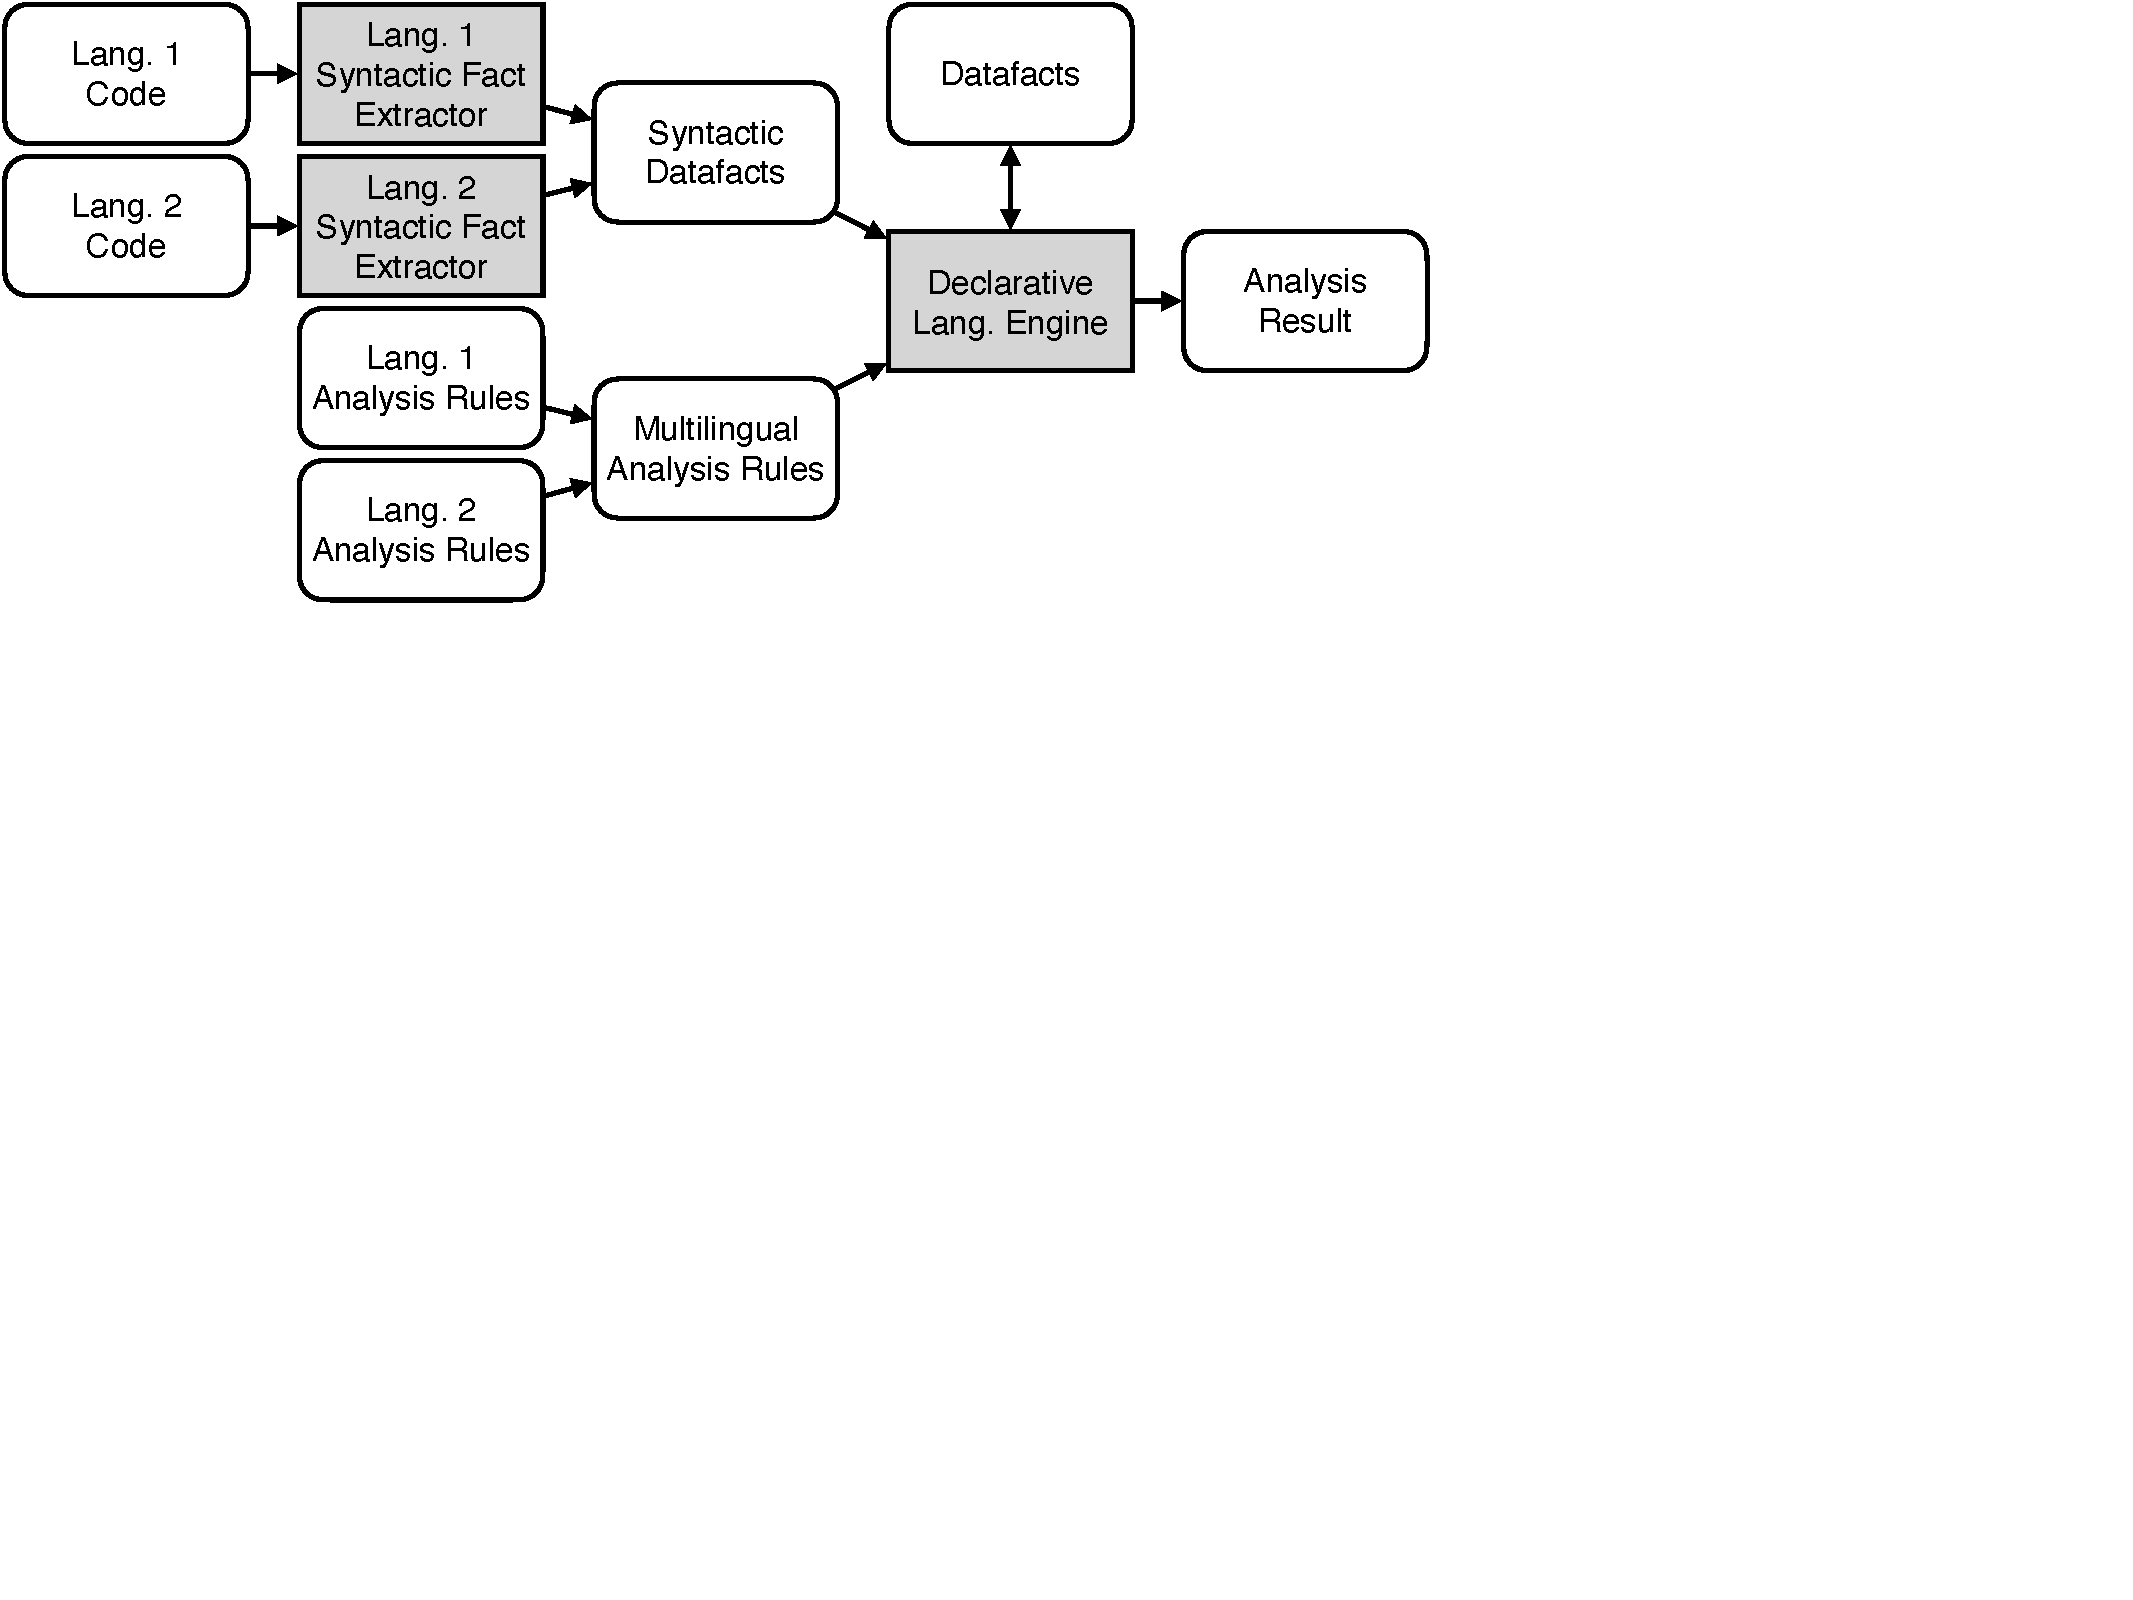
\includegraphics[width=0.5\textwidth]{img/overview2}

Above figure illustrate the overview of how declarative style analysis can be
extended to multilingual analysis. The main difference is that the evaluator
now gets two sets of syntactic data-facts extracted from both language, and the
rules also should be merged, with taking interoperation-semantics into account by
extending some rules.

In order to easily merge two sets of rules or each languages, two rules should
conform to the same framework, that is, they should have same sets of helper
data-facts (although the rule for deriveing helper data-facts might differ).
Given two sets of rules, the first thing to do id to identify the syntactic
parts of program where interaction can happen.  Then, based on the information
regarding these parts, new rules for generating proper helper data-facts are
defined, so that the interoperation semantic is properly modeled.

One thing to note here is that already-defined intra language rules for helper
data-facts and newly-defined inter-language rules can be treated independently;
defining new helper rules can be done without considering or modifying the 
previous implementation.

Let's illustrate this extension with the example of dataflow analysis above.
First, we are given two rules for the helper data-fact "step", for each language
respectviely:
\begin{lstlisting}[style=myDatalog,xleftmargin=2.5em]
step(a,b) :- step_A(a,b)
step(a,b) :- step_B(a,b)
\end{lstlisting}
In order to take the inter-language dataflow into account, one should find out
how a data of one language can be passed to different language beyond language
boudary.  One way to pass data in one language into another is via function
call, shown as in the example below:

\begin{lstlisting}[style=java,xleftmargin=2.5em]
public void main() { // Language A
  int x = SOURCE();
  B::f(x);
}
void f(int param) { // Language B
  printf("\%d", param);
}
\end{lstlisting}

Here, the variable x in language A is passed to the parameter of a function f
in language B. We can define the data-fact to reflect this kind of information,
foreignArgParam(a,b,i), which indicates that a is an i-th argument of a foreign
function call to a function whose i-th parameter is b. In above example, we
could derive the data-fact, foreignArgParam(x, param, 0). Using this data-fact,
we can add new rule for deriving the helper data-fact step as follows:
\begin{lstlisting}[style=myDatalog,xleftmargin=2.5em]
step(a,b) :- foreignArgParam(a,b,i)
\end{lstlisting}
so that dataflow through foreign dunction call also can be considered in this
framework.
